\subsection{Gruppe Arbejde}
\subsubsection{Organisering af gruppearbejde}

\paragraph*{Gruppekontrakt}
Som det første i projektet lavede vi en gruppekontrakt, 
hvori vi aftalte forholdene for dette projekt.
Et af de vigtigste forhold for gruppen var en forventningsafstemning, da alle gruppemedlemmerne havde tidligere haft uheldige oplevelser med gruppemedlemmer, der ikke havde samme forventninger som de andre i gruppen.
Heldigvis blev hele gruppen hurtigt enige om de fælles forventninger til projektet.
Derefter udvekslede gruppen kontaktoplysninger.
I gruppekontakten aftalte vi alt fra mødetid til konflikthåndtering.


I kontrakten aftalte vi at vi ville bruge OneDrive til deling af filer, Trello som scrumboard, Discord til intern kommunikation, Lucidchart til vores artefakter og GitHub til versionsstyring. 
Endvidere aftalte vi også at bruge Visual Studio som IDE.
Selve rapport blev skrevet i \LaTeX, da mange i gruppen havde haft en positiv oplevelse med det i tidligere projekter, og man kunne samtidig nemt tilføje og ændre ting i rapporten.

\paragraph*{Kvalitetssikring}
I gruppen lavede vi også en kvalitetsplan.
Idéen var, at vi fordelte alle de ting, som skulle kvalitetssikres: UML artefakterne og softwarekoden.
De forskellige artefakter blev så fordelt imellem gruppemedlemmerne, og gruppemedlemmet har så ansvaret for, at det tildelte artefakt var af en kvalitet, som hele gruppen ville kunne stå inde for.
Det betød ikke, at det var en selv, der skulle kvalitetssikre det, men det var det gruppemedlem, der skulle sikre, at kvalitetssikring skete for det artefakt.
Dette var en stor hjælp for gruppen, da hvert gruppemedlem fik ejerfornemmelser over deres tilgivne artefakter, og derfor var mere opmærksom på, at det var et ordenligt artefakt.

\paragraph*{Pairprogramming}
Under kodning gjorde vi stor brug af pairprogramming, dette hjalp med at mindske fejl, sikrede for bedre løsninger og gav os en større produktivitet.
Ud over dette aftalte vi i gruppen at efter noget er blevet lavet, 
skal det reviewes af et andet medlem i gruppen, før det kan kvalificeres som færdigt. Vi opholdte reglen ved at opsætte regler i Github, der gjorde det umuligt at lave et merge uden et pull-request.

\subsubsection{Kontakt med virksomhed}

Vi fik etableret tidlig kontakt med vores virksomhed, da vi var tidlig ude og søge virksomhed.
En af virksomhederne vi kom i kontakt med var så Psykolog Nord.
Vi mødtes med dem den 27 februar, hvor de præsenterede deres problem, og vi kunne præsentere, hvad formålet med vores eksamensprojekt var.

Projektet blev godkendt af underviserne, hvorefter vi aftalte et møde den 25 marts, før pre-sprinten, hvor PsykologNord havde lavet en oversigt over de problemer de har i deres hverdag.
Til mødet diskuterede vi også frem og tilbage, hvad vi mente var realistisk, at vi ville kunne lave; bl.a. er udvikling af hjemmesider og smart-phone apps uden for førsteårspensum.
Desuden fik vi også planlagt de møder, som vi ville have i løbet af projektforløbet.

Vi aftalte at holde møder med dem hver anden uge, hvor vi præsenterede, hvad vi havde nået, de kunne komme med input på projektet, og vi kunne få svar på spørgsmål som evt. var opstået siden sidste møde.

Det var bevidst, at der skulle være møder hver anden uge, da vores scrum sprints varede 2 uger hver.

Møderne har hjulpet gevaldigt med at sikre udvikling i den rigtige retning, dertil fjernede de tvivl omkring den ønskede adfærd af systemet, der opstod undervejs, og vi kunne også omprioritere undervejs, da vi opdagede, at vi ikke ville kunne nå alt det, som vi talte om til mødet den 25 marts.

\subsubsection{Kodestruktur}

Undervejs i projektet har vi som gruppe taget mange beslutninger omkring koden.
Kodestandarder, lagdeling og patterns er alle blev brugt. 

Da vi skulle kode aftalte vi at, udvikle programmet ved brug af top-down udvikling.
Vi skulle derfor udvikle fra UI-laget og så langsomt gå ned i lagene, som vi udviklede.
Det gjorde at vi kun inkorporerede det nødvendige i hver klasse, og kun gav nødvendige relationer, og på den måde har det også hjulpet os med at overholde GRASP og SOLID principperne.

Vi valgte at bruge top-down udvikling, da vi tidligt i forløbet blev enige med PO om, hvordan vores UI skulle se ud, og vi derfor tidligt også kunne implementere vores WPF-vinduer, som vi også beskriver i \ref{GUI}.

Noget af det vi fik ud af det var at vi hele tiden kunne køre en funktion i programmet helt igennem fra at der bliver trykket på en knap i UI'et til at der sker en reaktion i databasen, hvilket har gjort at vi har haft en masse små succes oplevelser, som har holdt vores arbejdsmoral oppe.
En af de negative effekter er dog, at vi har et UI, hvor det ligner, at man kan en helt masse mere end er muligt, hvilket nok har fået vores PO til at tro, at vi nåede meget mere, end vi gjorde.
Alt i alt synes vi dog, at det har været en gevinst at bruge denne form for udvikling, når vi netop havde vores færdige UI så tidligt i forløbet.

\subsubsection{Scrum og retrospektiver}

Vi valgte at køre to ugers sprints, da vi følte, at dette passede bedst med størrelserne af vores PBI'er og mødetiderne med vores PO ifht. sprintreviews.

\paragraph*{Scrumboard}
Til at hjælpe os med at organisere vores arbejde har vi brugt Trello som scrumboard.
På vores scrumboard havde vi fem felter:
\begin{enumerate}
    \item Product Backlog Items, der indeholdt alle de backlog items, som vi skulle nå i projektet.
    \item To Do, hvad der skulle arbejdes med i denne sprint.
    \item Doing, hvad der arbejdes med lige nu.
    \item Review, hvad der skal kvalitetssikres af andre gruppemedlemmer.
    \item Done, hvad der er færdigt i denne sprint.
\end{enumerate}

På Trello kan man tilføje sig på en task, så når et gruppemedlem flyttede en task fra To Do til Doing satte han sig på tasken, så vi kunne se, hvem der var igang med hvad.

\paragraph*{Planning poker}
I begyndelsen af hver sprint brugte vi planning poker til at vurdere hvor lang tid hver af de forskellige opgaver under sprinten ville tage.
Det gjorde det nemmere at se og vurdere vores fremskridt i sprintet, også selvom man nogen gange vurdere tidsforbruget på opgaven forkert.
Vi kan konstatere, at ingen af os er gode til planning poker endnu, da vi ofte skød flere timer forkert, men vi er forhåbningsfulde om, at det bliver vi bedre til med tiden.
I løbet af projektforløbet blev vores bud på hvor meget tid en opgave ville tage mere præcis, da vi fik noget at sammenlige med.

\paragraph*{Standup meeting}
Vi startede hver dag med et kort stand up meeting, hvor hvert gruppemedlem fortalte, hvad de havde tænkt sig at arbejde med den dag, hvad de arbejdede med dagen forinden, og om der er noget der forhindrer dem i komme videre med deres arbejde.
Derved sikrede vi alle havde en opgave at gå i gang med, og alle havde et godt overblik over status af projektet.
Den sidste uge af projektet, der gik med det sidste rapportskrivning kom vi til at glemme stand up meetingsne i de første par dage, hvilket betød, at et gruppemedlem sagde tirsdag aften, at han havde mistet overblikket over, hvor langt vi var nået.
Det var altså tydeligt at se, at det var vigtigt at vi holdte vores morgenmøder, som vi så også holdt de sidste dage i projektforløbet igen.

\paragraph*{Sprint retrospektiver}
Efter hvert sprint holdte vi et sprint retrospektiv. Her skiftede vi altid roller, så det ikke var den samme person der var scrum-master.
I vores sprint retrospektiver blev der talt om, hvad vi synes var gået godt, og hvad vi synes var gået mindre godt.
Til det første sprint review gjorde to gruppemedlemmer opmærksom på, at de synes de to andre gruppemedlemmer havde været slemme til at kaste sig over koden og overlade de mindre spændende opgaver til dem.
Efter det retrospektiv blev hele gruppen mere opmærksom på at have en bedre fordeling af arbejdstyperne, og vi havde ikke det problem i resten af projektet.
Det er vigtigt, at hvert gruppemedlem er ærlig om, hvad de synes er gået mindre godt, og hvad de synes skal gøres bedre i det næste sprint, da ellers kan man ikke få løst problemerne, der opstår i forløbet.

\paragraph*{Happiness index}
Efter hver uge i projektet kørte vi et happiness index for hver person.
Det havde vi internt i gruppen valgt at bruge, for at have en status over, hvordan folk syntes projektet gik, og om de havde evt. grunde til deres happiness.
Ens happiness, som gik på en skala 1-5, kunne være alt fra noget projektrelateret til bare hvorledes man havde det.

\begin{figure}[h]
    \caption{Graf for Happiness index}
    \centering
        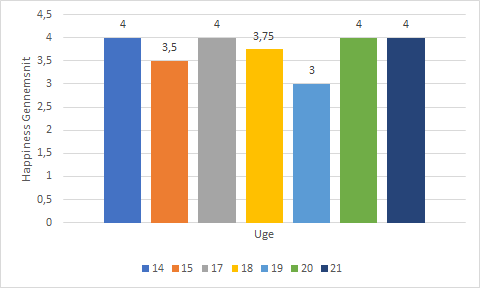
\includegraphics[scale=0.90]{HappinessIndex.png}
    \label{happinessindex}
\end{figure}

Meget at tiden var der en positiv morale i gruppen.
De eneste bemærkelsesværdige uger var uge 15 og uge 19.
I uge 15 var happinessen nede, da koncentrationen ikke var så stærk som i den tidligere uge, og vi derfor var irriterede på os selv og bekymrede for, hvad der skulle ske, hvis denne mangel på koncentration ville fortsætte.
Heldigvis var der ikke mangel på koncentration i de resterende uger.
I uge 19 var happinessen nede pga. vi fik besked på at undervisningsholdene vil blive splittet.
Ud over det var alle meget tilfredse med arbejdet i projektet.

\subsubsection{Burndownchart}

Under hele projektet har vi forsøgt at notere vores tidsforbrug ved brug af et burndownchart.
Sammen med planning poker giver det os et overblik over, hvordan sprinten forløber, og om evt. justering. 

Efter hvert sprint tog vi et billede af burndowncharten og opstillede en ny for den næste sprint.
På den måde havde vi et burndownchart for hvert sprint, så vi kunne se fremskridtet for hver sprint.

En af de gennemgående temaer i vores burndowncharts er dog tilføjelser til sprinten.
Vi fandt ofte ud af, at der også var en anden opgave som skulle gøres under sprinten, som så gjorde at flere timer blev tilføjet til burndowncharten midt-sprint. 

Dette kan f.eks. ses i pre-sprinten på figur \ref{fig:burndownpresprint}.
Først gik det godt med at følge den ideelle burndown, men midtvejs opstår der problemer, da vi opdagede, at der skulle laves noget mere og tingene går lidt i stå.

\begin{figure}[h]
    \caption{Burndownchart for presprinten}
    \centering
        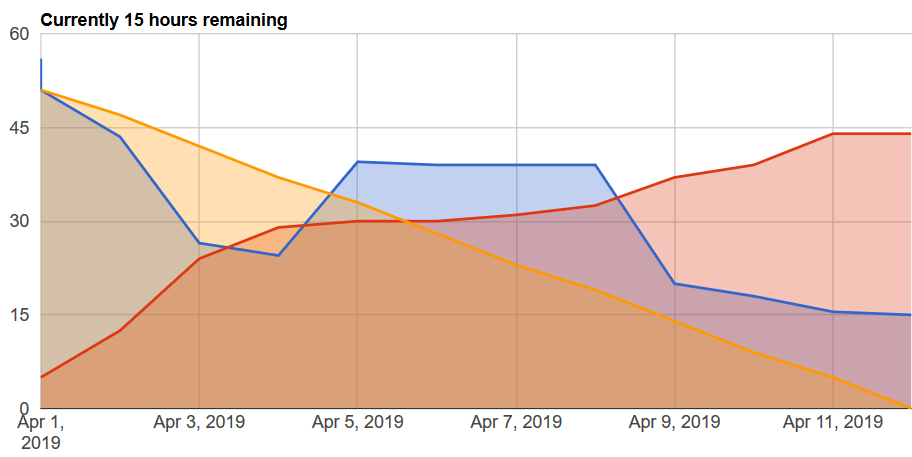
\includegraphics[width=\textwidth]{Burndownchart_PreSprint.png}
    \label{fig:burndownpresprint}
\end{figure}

I sprint 1 se figur \ref{fig:burndownfirstsprint} overholdes den ideelle burndown mere.
I denne havde vi også bedre overblik over hvad der skulle gøres, takket være hvad vi lærte i pre-sprinten, samt bedre overvejelse ved planlægningen.
Vi havde dog undervurderet implementering af vores PBI, som gjorde at vi gik i stå til sidste i sprinten, og disse PBI'er blev overført til næste sprint.

\begin{figure}[h]
    \caption{Burndownchart for første sprint}
    \centering
        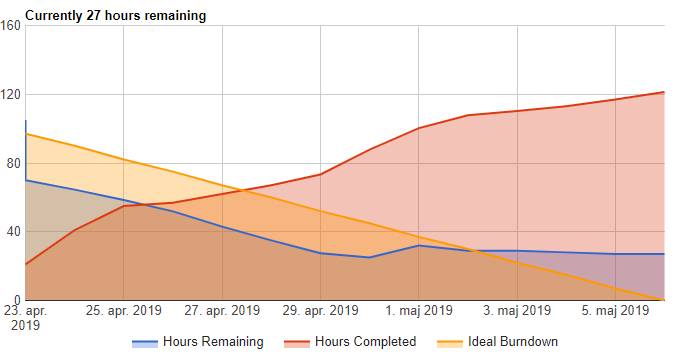
\includegraphics[width=\textwidth]{Burndownchart_1.png}
    \label{fig:burndownfirstsprint}
\end{figure}

Vores anden sprint blev ramt af problemerne fra sprint 1 se bilag \ref{bilag:burndownsecondsprint} side \pageref{bilag:burndownsecondsprint}, som betød den blev opdateret lidt sent.
Det betød, at burndownchartens mængde af timer brugt ændrede sig midt i sprinten.
Vi havde dog stadig en produktiv sprint, hvor vi nåede en større del af opgaverne.



\subsubsection{Erfaringer i projektet}

Undervejs har der opstået problemer i projektet.
Et eksempel var da et gruppemedlem kom til at merge ind på masteren med en branch, som ikke var up-to-date, hvilket betød meget af koden i masteren blev ændret.
Heldigvis blev det indset med det samme og mergen blev reverted.
På den måde fandt vi også ud af at vores Github regler var forkert sat op.
Det blev så fikset.

Et mere alvorligt problem var, da et gruppemedlem manglede filer efter at have merged to branches.
I forsøget på at løse dette problem mistede begge branches kode, som så skulle genskrives.
Heldigvis var koden skrevet på samme dag, så da de manglende dele var fundet var det ikke for svært at skrive igen.
Hertil lærte vi så at Github ikke cloner alt med hver eneste gang du henter en branch ned.
Derimod ved vi nu at det altid er en god ide at rebuilde en solution, og være meget opmærksom på, at man har alle de filer, som man bør have.